\documentclass[aspectratio=169]{beamer}
%package
\usepackage[utf8]{inputenc}
\usepackage[T1]{fontenc}
\usepackage{tikz}
\usepackage{appendixnumberbeamer}

\usetheme[showmaxslides,darkmode]{pureminimalistic}
\definecolor{title}{RGB}{51, 255, 119}

\renewcommand{\beamertitlecolor}{title}
\renewcommand{\appendixname}{\texorpdfstring{\translate{appendix}}{appendix}}
% no logos
\renewcommand{\logofooter}{}
\renewcommand{\logotitle}{}
\renewcommand{\logoheader}{}

\title[Portfolio] {Portfolio}
\author{Emmanuel Vera}
\institute{Senior Electronics Engineer}
\date{\today}


\begin{document}

\maketitle

\begin{frame}[plain, noframenumbering]{Outline}
  \tableofcontents
\end{frame}

\section{Projects}

\begin{frame}{Mastrack}
  OBD interface car sensor board that records and transmit geo-data. It uses a 
  STM32 microcontroller and a BG95 quectel module.
  \begin{figure}[H]
    \centering
    \begin{columns}[T]
      \begin{column}{.5\linewidth}
        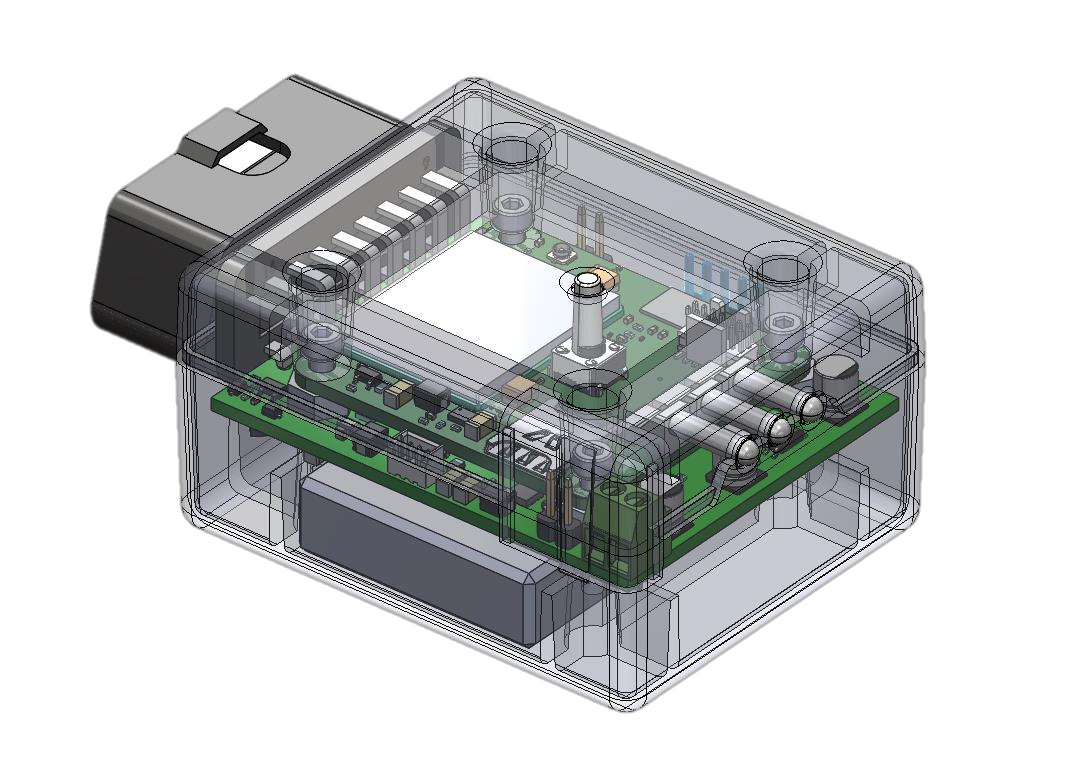
\includegraphics[width=\linewidth]{images/Mastrack1}
      \end{column}
      \begin{column}{.5\linewidth}
        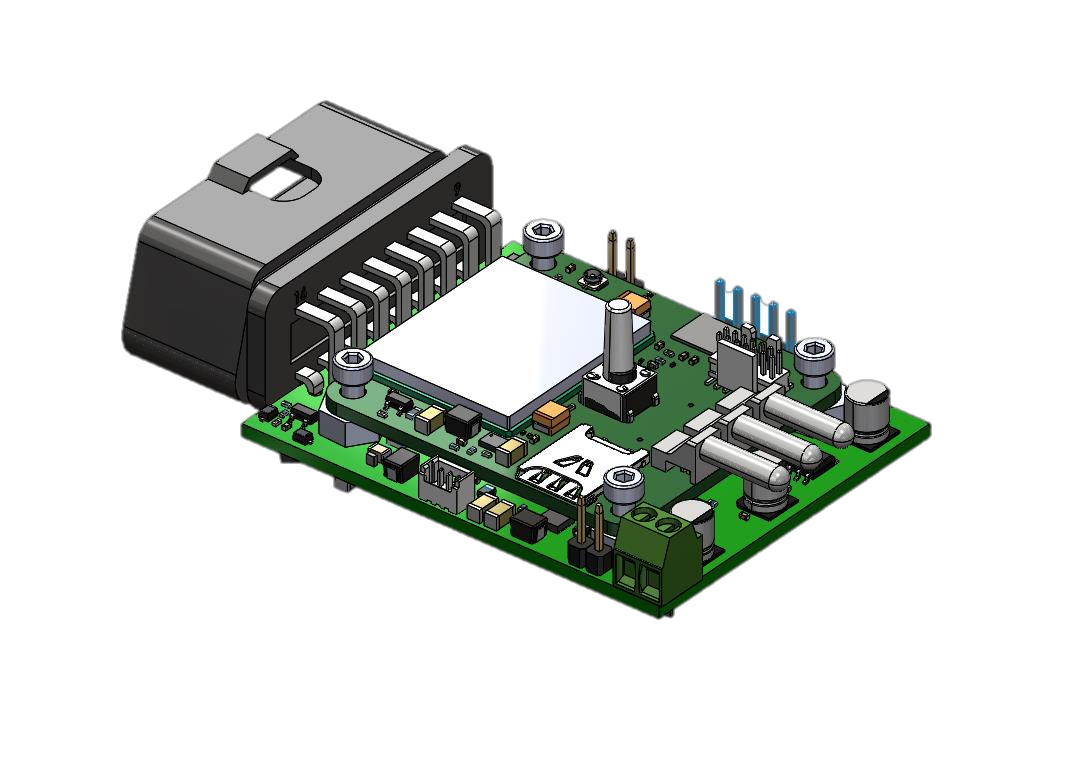
\includegraphics[width=\linewidth]{images/Mastrack2}
      \end{column}
    \end{columns}
  \end{figure}
\end{frame}

\begin{frame}{Bacnet door holder}
  IoT WiFi control system for doors in public places through the bacnet
  protocol and using and electro magnet. The device works with a PIC18F47J53 
  and an ESP8266 as main microcontrollers and it is connected to the BacNet 
  server to be configured.

  \begin{figure}[H]
    \centering
    \begin{columns}[T]
      \begin{column}{.24\linewidth}
        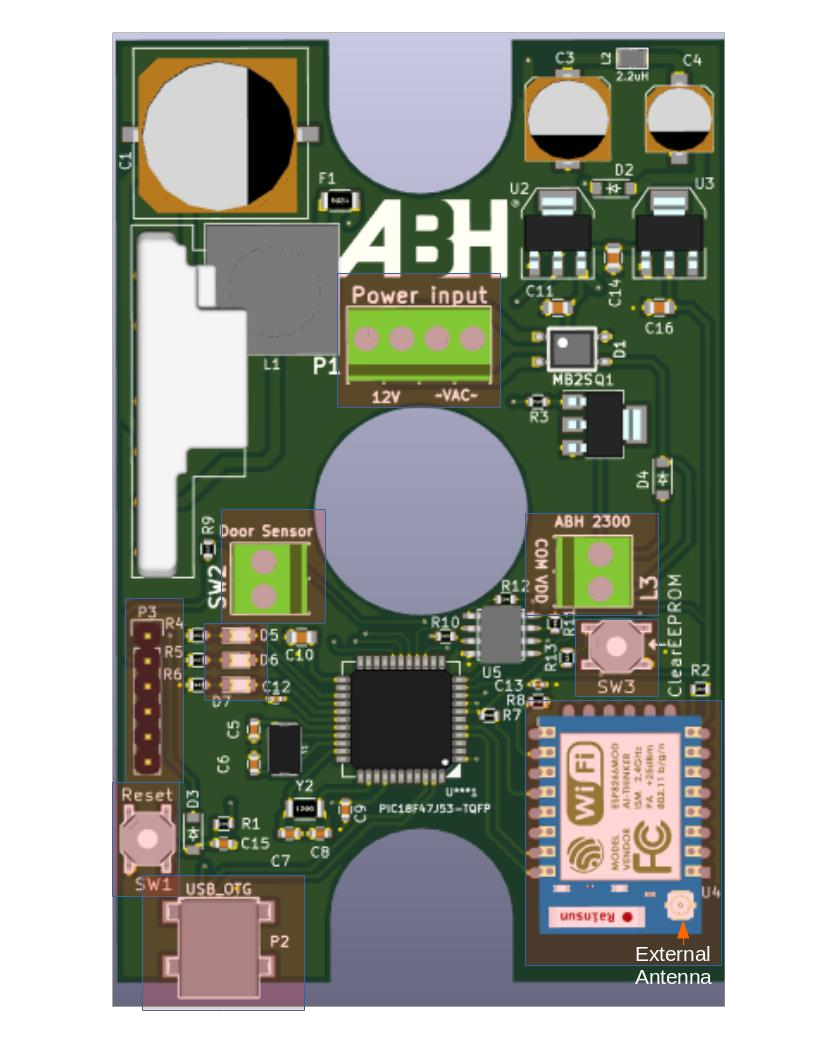
\includegraphics[width=\linewidth]{images/BacnetDoorHolder1}
      \end{column}
      \begin{column}{.2\linewidth}
        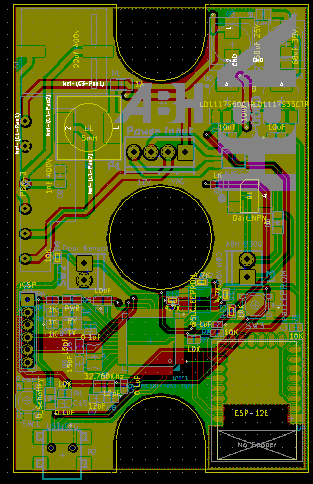
\includegraphics[width=\linewidth]{images/BacnetDoorHolder2}
      \end{column}
    \end{columns}
  \end{figure}
\end{frame}

\begin{frame}{Bluetooth phonogram}
  Battery powered bluetooth speaker with phonogram shape designed with a BM64
  microchip audio bluetooth module.
  \begin{figure}[H]
    \centering
    \begin{columns}[T]
      \begin{column}{.3\linewidth}
        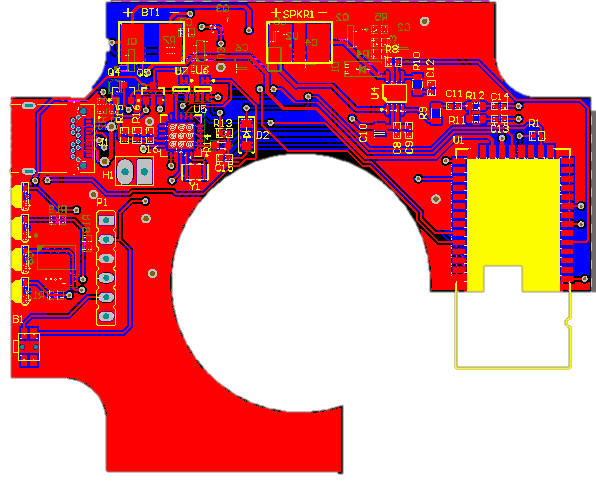
\includegraphics[width=\linewidth]{images/BluetoothPhonogram1}
      \end{column}
      \begin{column}{.3\linewidth}
        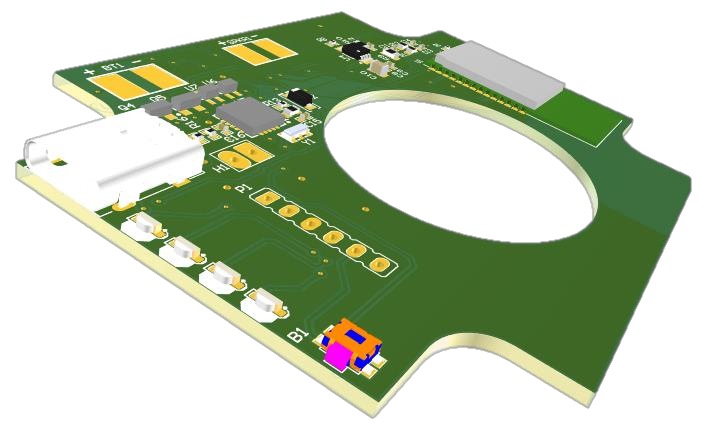
\includegraphics[width=\linewidth]{images/BluetoothPhonogram2}
      \end{column}
      \begin{column}{.3\linewidth}
        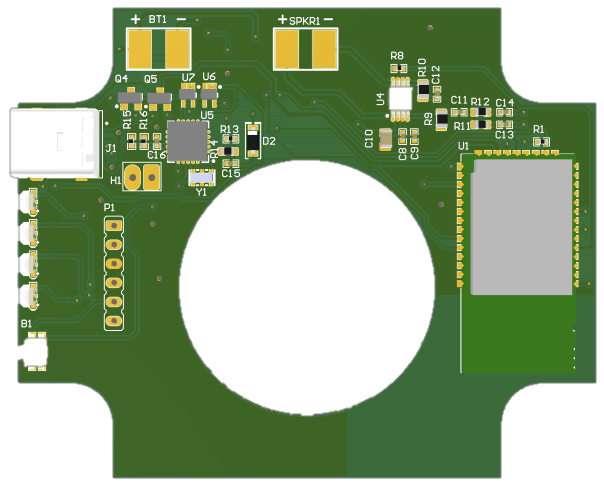
\includegraphics[width=\linewidth]{images/BluetoothPhonogram3}
      \end{column}
    \end{columns}
  \end{figure}
\end{frame}

\begin{frame}{Elevated plus maze automation}
  Control system for an automated maze used in research laboratories with the
  purpose of develop anxiety drugs. It uses a microchip microcontroller as main
  controller, touch screen, HC-05 bluetooth module, esp8266 WiFi module and 
  VDrive module to store data in USB pendrives.

  \begin{figure}[H]
    \centering
    \begin{columns}[T]
      \begin{column}{.3\linewidth}
        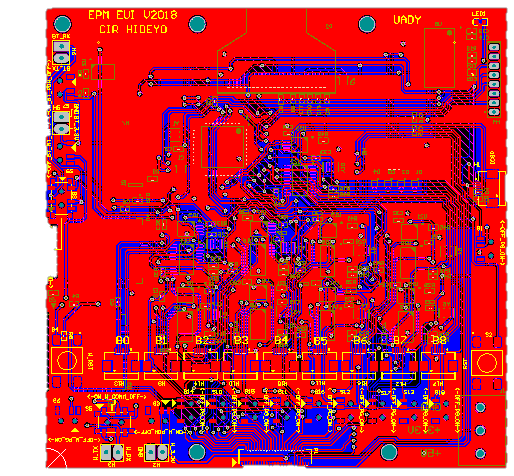
\includegraphics[width=\linewidth]{images/EPM-auto1}
      \end{column}
      \begin{column}{.3\linewidth}
        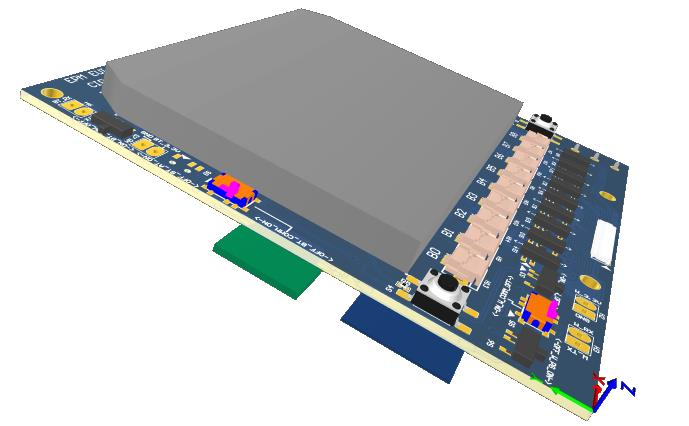
\includegraphics[width=\linewidth]{images/EPM-auto2}
        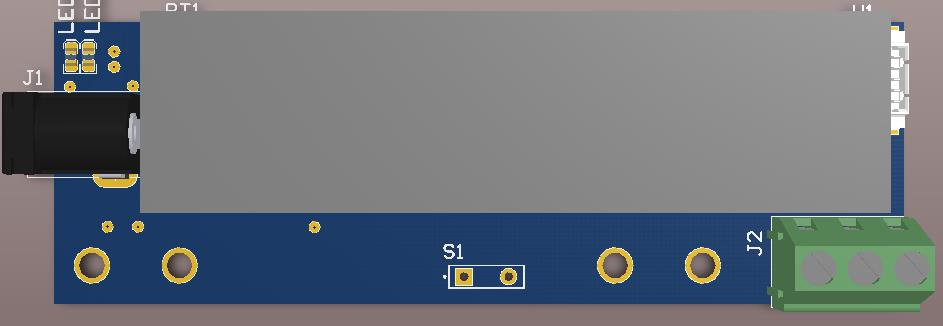
\includegraphics[width=\linewidth]{images/EPM-auto3}
      \end{column}
      \begin{column}{.3\linewidth}
        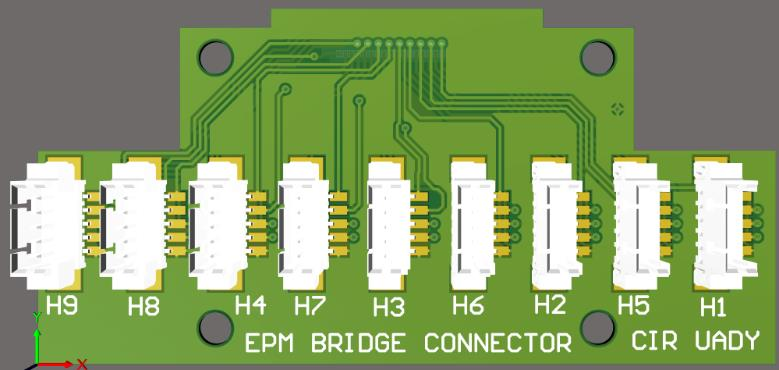
\includegraphics[width=\linewidth]{images/EPM-auto4}
        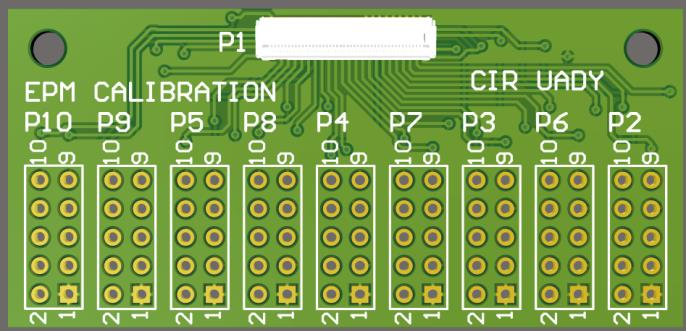
\includegraphics[width=\linewidth]{images/EPM-auto5}
      \end{column}
    \end{columns}
  \end{figure}
\end{frame}

\begin{frame}{iSparkle Light}
  Electronics for a musical and light demo display for a Christmas lightning
  product. It uses a ATmega microcontroller and audio module.
  \begin{figure}[H]
    \centering
    \begin{columns}[T]
      \begin{column}{.5\linewidth}
        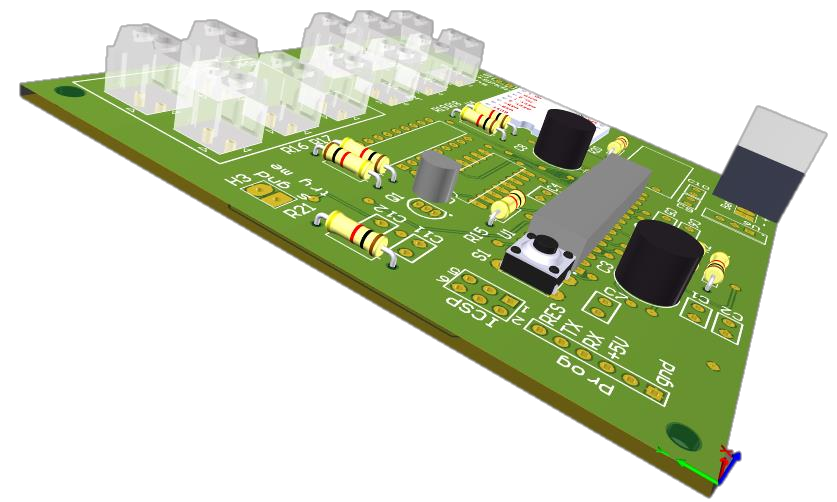
\includegraphics[width=\linewidth]{images/isparkle1}
      \end{column}
      \begin{column}{.3\linewidth}
        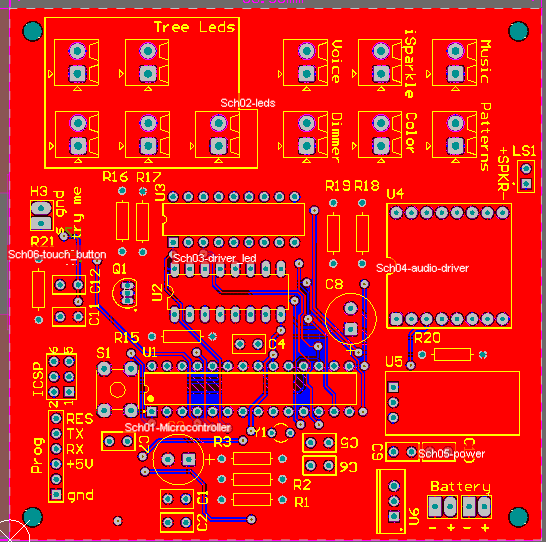
\includegraphics[width=\linewidth]{images/isparkle2}
      \end{column}
    \end{columns}
  \end{figure}
\end{frame}

\begin{frame}{Telemetry logger}
  Telemetry data logger that stores and sends data through a GPRS module.
  It is commonly used for industrial meters. It uses a SIM900 module and a
  Microchip microcontroller as its main controller.
  \begin{figure}[H]
    \centering
    \begin{columns}[T]
      \begin{column}{.3\linewidth}
        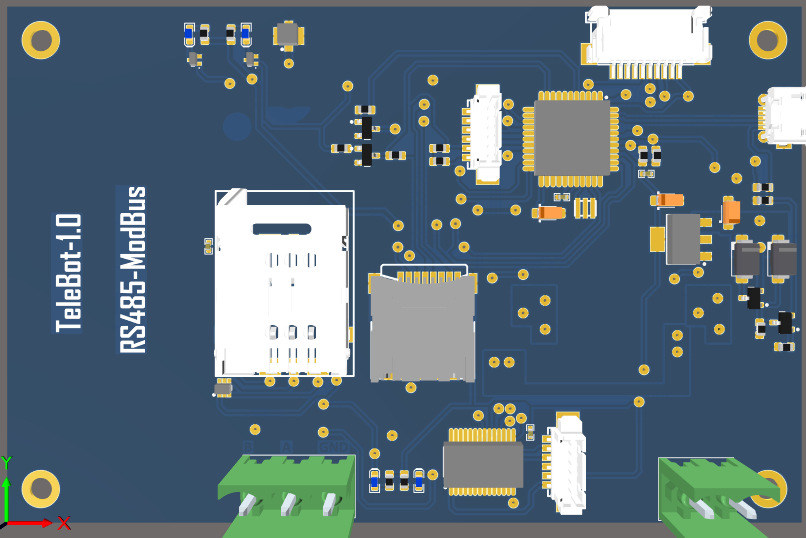
\includegraphics[width=\linewidth]{images/telebot1}
      \end{column}
      \begin{column}{.3\linewidth}
        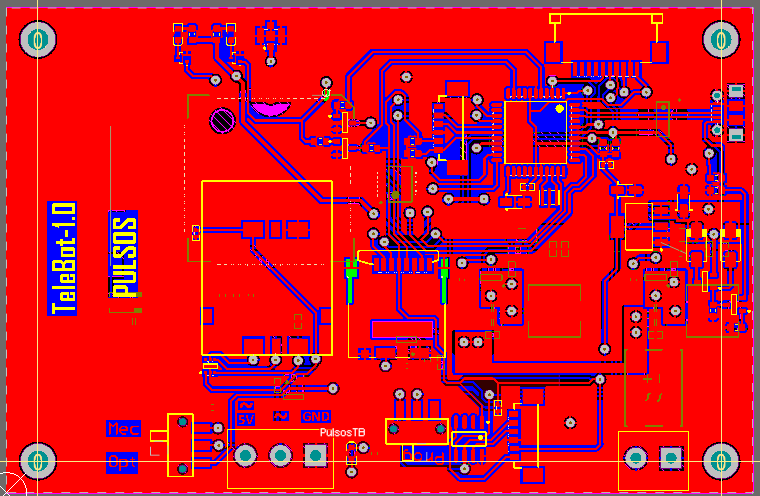
\includegraphics[width=\linewidth]{images/telebot2}
      \end{column}
      \begin{column}{.3\linewidth}
        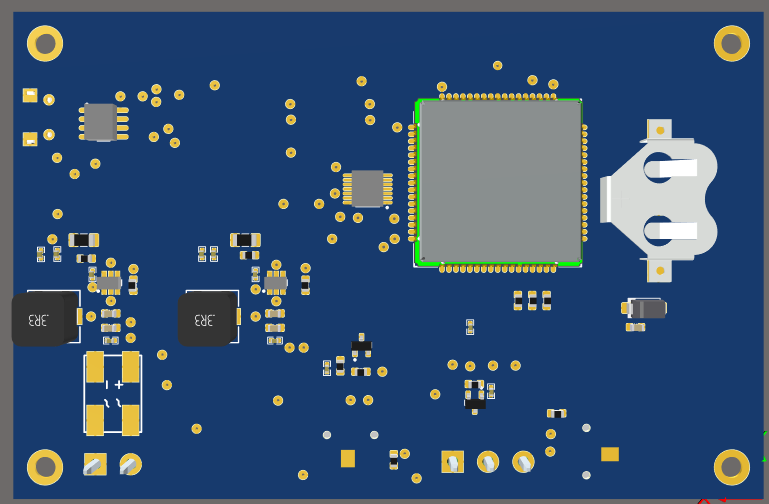
\includegraphics[width=\linewidth]{images/telebot3}
      \end{column}
    \end{columns}
  \end{figure}
\end{frame}

\begin{frame}{WDS}
  This device turns on/off washing machines and receive commands from 
  AWS IoT services. It is used to rent washing machines for a certain pre-paid
  time. It uses a ESP32 as its main microcontroller.
  \begin{figure}[H]
    \centering
    \begin{columns}[T]
      \begin{column}{.4\linewidth}
        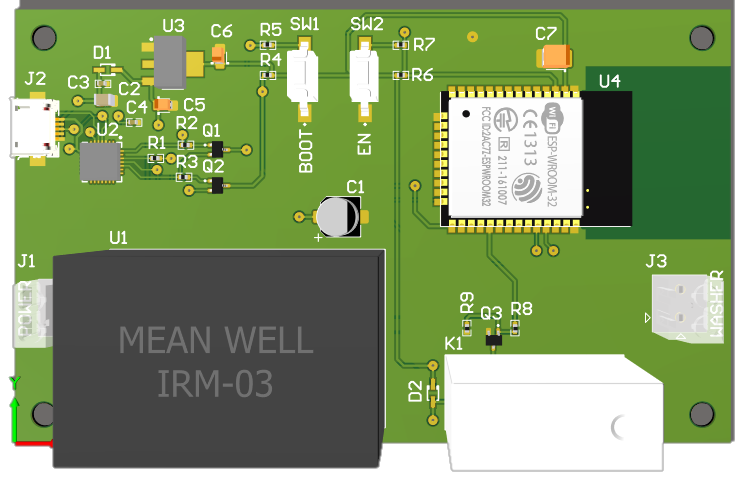
\includegraphics[width=\linewidth]{images/wds1}
      \end{column}
      \begin{column}{.4\linewidth}
        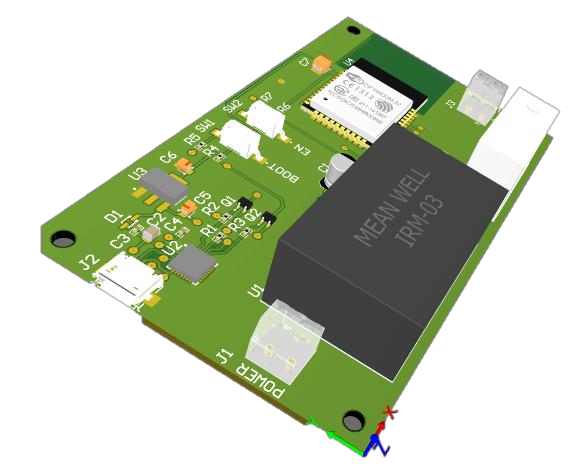
\includegraphics[width=\linewidth]{images/wds2}
      \end{column}
    \end{columns}
  \end{figure}
\end{frame}

\section{SKILLS}
\begin{frame}{Skills}
  \begin{itemize}
    \item Electronics Design (Altium)
    \item PCB Design (Altium)
    \item PCB assembly for prototyping
    \item IoT related Software/Firmware Development
  \end{itemize}
\end{frame}

\end{document}
